
\subsection{Data Preprocessing}
\label{Subsect:Data-preprocessing}

stopword removal, etc. for standard classifiers
No stopword removal for CNN

\subsection{Initial Experiments with Business Unit 1 dataset}
\label{Subsect:BU1-exp}

\begin{wrapfigure}{l}{0.75\textwidth}
\centering
\subfloat[{BU1 prediction using Word Unigram Count features}]{\label{Figure_BU1-WUC}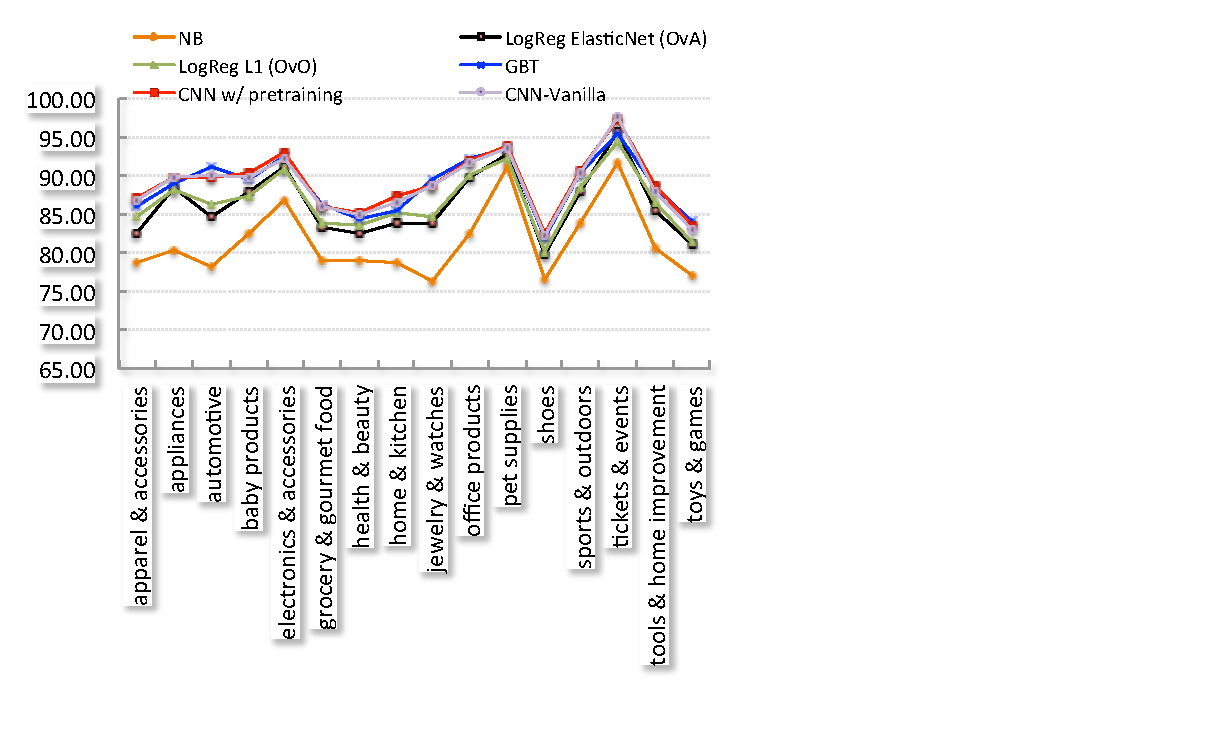
\includegraphics[width=0.35\textwidth]{images/BU1-WUC-predictions}} \hspace{0.01cm}
\subfloat[{BU1 prediction using Word Unigram BiPositional Count features}]{\label{Figure_BU1-WUBPC}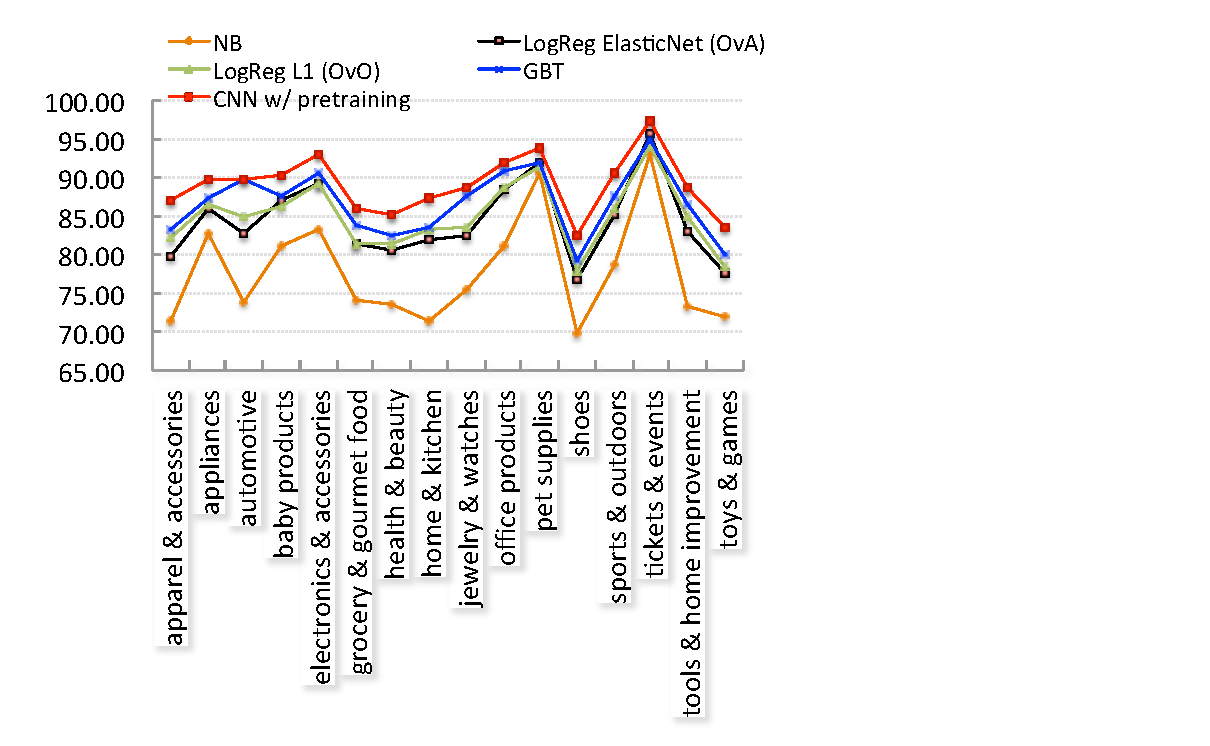
\includegraphics[width=0.35\textwidth]{images/BU1-WUBPC-predictions}} 

\subfloat[{BU1 prediction using Word Bigram Count features}]{\label{Figure_BU1-WBC}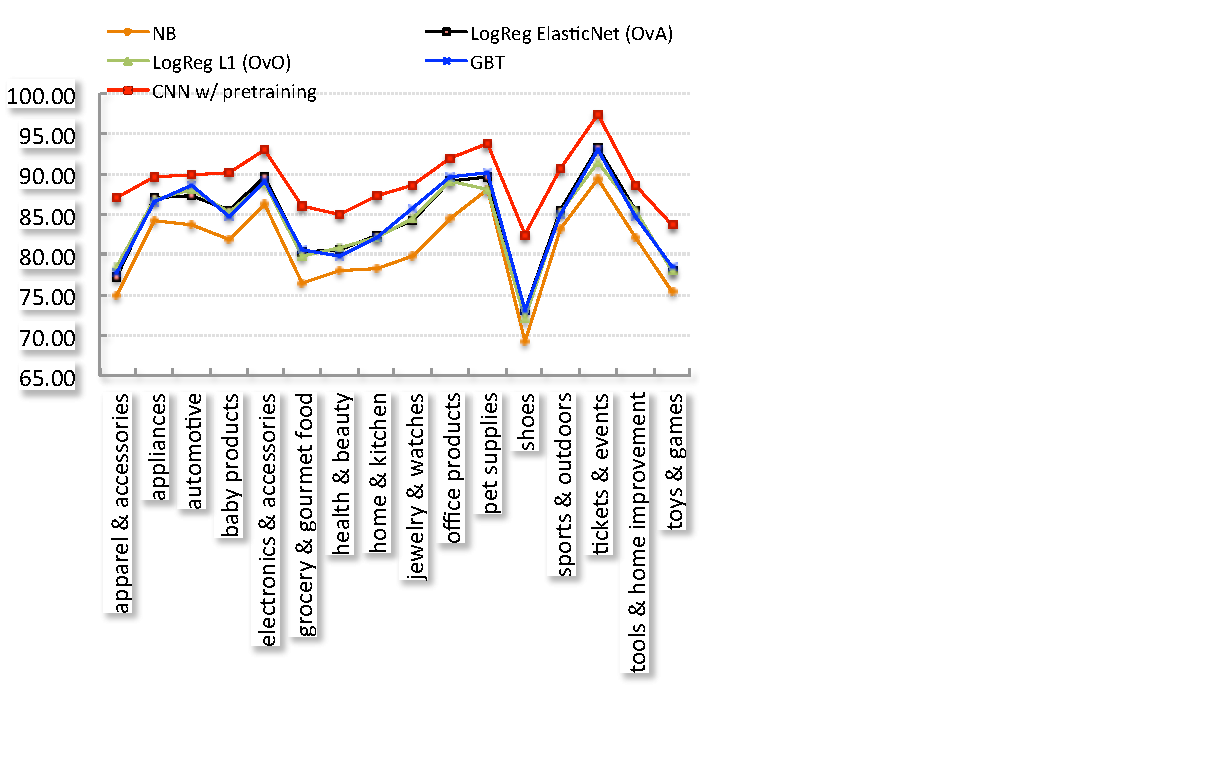
\includegraphics[width=0.35\textwidth]{images/BU1-WBC-predictions}} \hspace{0.01cm}
\subfloat[{BU1 prediction using Word Bigram Bi Positional Count features}]{\label{Figure_BU1-WBBPC}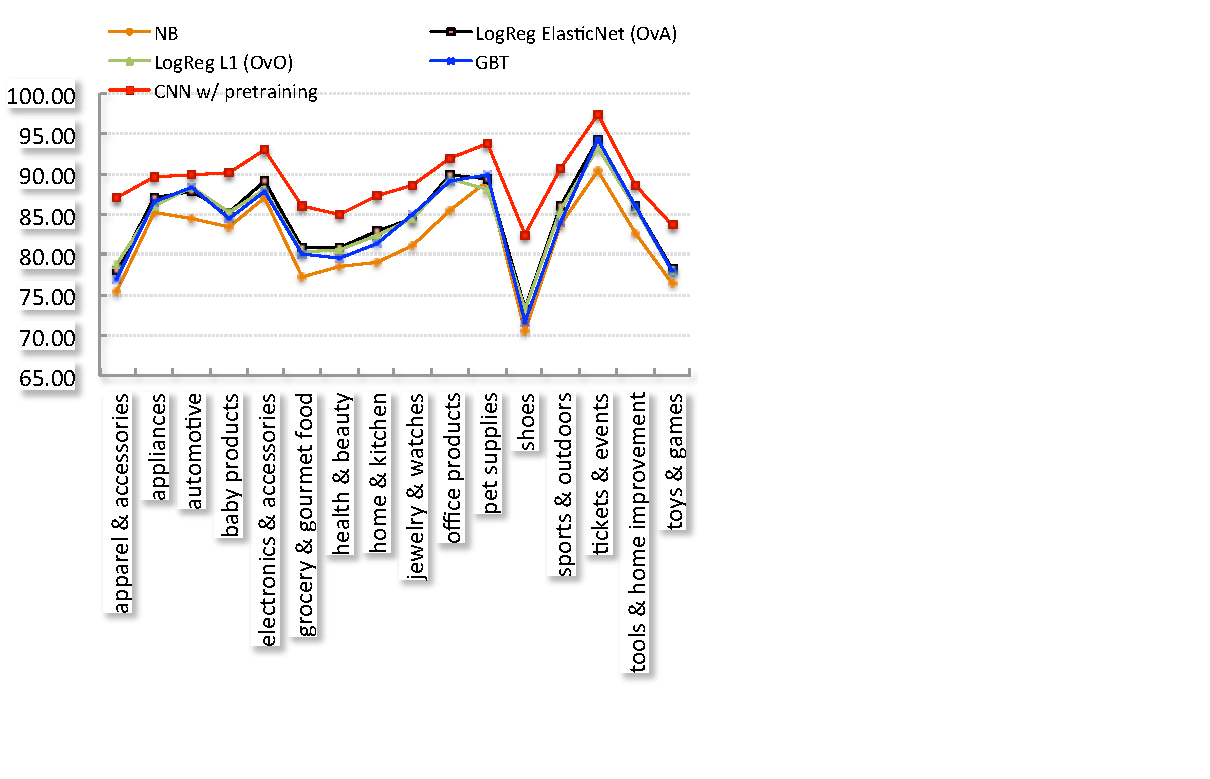
\includegraphics[width=0.35\textwidth]{images/BU1-WBBPC-predictions}} 
\caption{{Predictions on Business Unit 1 test set} }
\label{Figure_BU1-predictions}
\end{wrapfigure}

\begin{wrapfigure}{r}{0.4\textwidth}
\centering
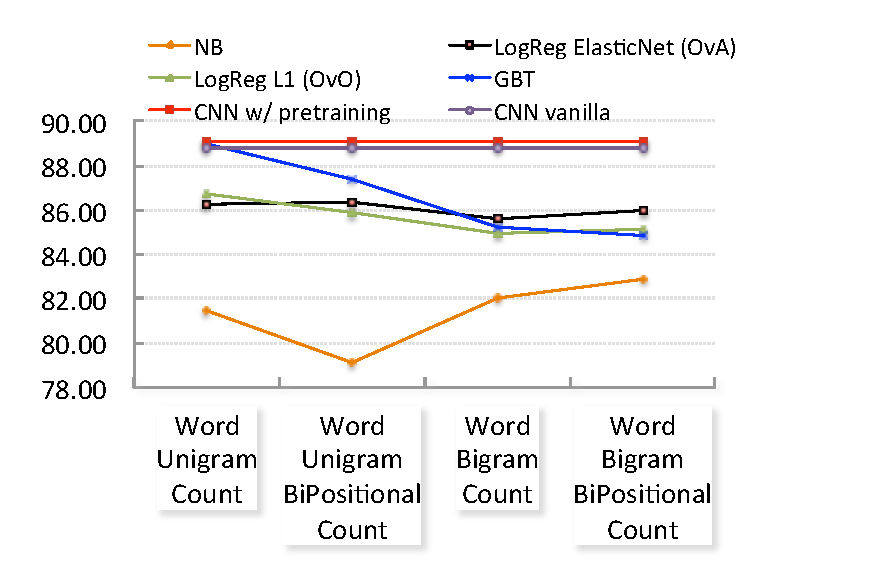
\includegraphics[width=0.35\textwidth]{images/BU1-mean-micro-precision}
\label{Figure_BU1-predictions-feature-averages}
\end{wrapfigure}

\subsection{Noise Analysis of Business Unit 2 Dataset using Correspondence LDA}
\label{Subsect:BU2-noise-analysis}
